\subsection{Realimentación en un amplificador}

Los primeros amplificadores operacionales fueron implementados con tubos de vacío, en computadores analógicos para resolver operaciones matemáticas complejas, combinando la ganancia y la realimentación negativa.

En 1968 se introdujo el $\mu A741$, como el primer amplificador estándar en la industria electrónica.

Un amplificador es un dispositivo que tiene dos puertods de entrada, llamados puerto inversor y puerto no inversor, y una salida que es proporcional
al valor de la entrada por una ganancia.

Un amplificador $\mu$741 tiene una ganancia típica de 200V/mV , o 106dB. Sin embargo, esta ganancia se sostiene en un pequeño ancho de banda cuando el amplificador no está realimentado.

Suponga que tenemos un amplificador con ganancia A, como se observa
en la figura \ref{fig:mt-amplificador-sin-realimentar}.

\begin{figure}[ht]
    \centering
    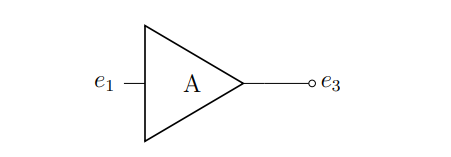
\includegraphics[width=0.5\textwidth]{src/images/amplificador-sin-realimentar.png}
    \caption{Amplificador sin realimentación}
    \label{fig:mt-amplificador-sin-realimentar}
\end{figure}

\begin{figure}[ht]
    \centering
    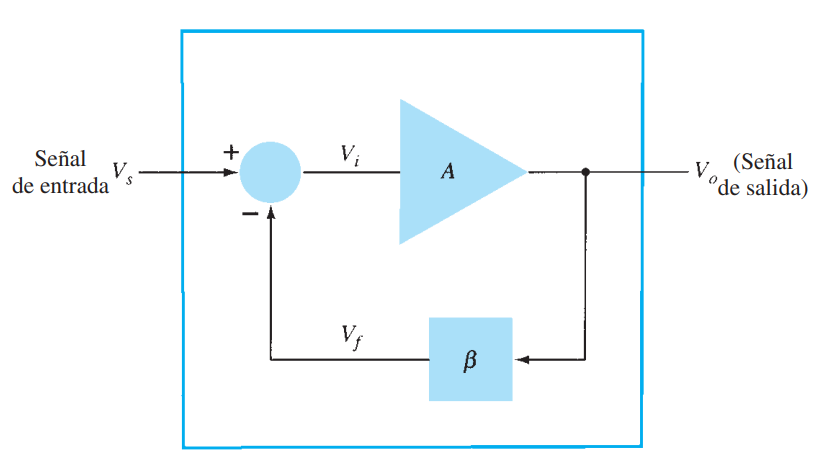
\includegraphics[width=0.5\textwidth]{src/images/amplificador-realimentado.png}
    \caption{Diagrama de bloque del amplificador realimentado}
    \label{fig:mt-amplificador-realimentado}
\end{figure}

Y este amplificador se realimenta con una red de ganancia $\beta$ como se muestra en la figura \ref{fig:mt-amplificador-realimentado}. Entonces podemos definir el siguiente sistema de ecuaciones:

\begin{align*}
    v_o & = e_1 \cdot A \\
    e_1 & = v_i + \beta v_o \\
    e_o & = v_o
\end{align*}

Resolviendo este sistema de ecuaciones, encontramos la siguiente función de transferencia:

\begin{equation}
    \boxed{A_{fb} = \frac{v_o}{v_i} = \frac{A}{1 - \beta A}}
    \label{eq:mt-func-transferencia-realimentacion}
\end{equation}

De esta ecuación podemos definir cinco zonas:

\begin{align*}
\text{Realimentación negativa o degenerativa:} & \quad \beta A < 0 \\
\text{Realimentación positiva o regenerativa:} & \quad 0 < \beta A < 1 \\
\text{Realimentación nula:} & \quad \beta A = 0 \\
\text{Oscilación:} & \quad \beta A = 1 \\
\text{Inestabilidad:} & \quad \beta A > 1
\end{align*}

\subsection{Método del amplificador desvanecido (MAD)}

 El método aprovecha las características reales del
amplificador operacional para desvanecer los elementos no lineales, de manera que el problema se reduce a resolver un sistema compuesto de elementos pasivos.

Supongamos que tenemos un sistema que está realimentado, entonces encontramos el lazo de realimentación que contiene al amplificador principal,
y encontramos los siguientes parámetros, para resolver la ecuación de la ganancia.


\begin{align*}
    x_{io} = \left. \frac{v_o}{v_i} \right|_{A=0} \\
    x_{i1} = \left. \frac{e_1}{v_i} \right|_{A=0} \\
    x_{3o} = \left. \frac{v_o}{e_3} \right|_{v_i=0} \\
    x_{31} = \left. \frac{e_1}{e_3} \right|_{v_i=0}
\end{align*}

donde

\begin{itemize}
    \item $x_{io}$ es la ganancia vista desde la entrada $v_i$ hasta $v_o$ con el amplificador
desvanecido.
    \item $x_{i1}$ es la ganancia vista desde la entrada $v_i$ hasta $e_1$ con el amplificador \
desvanecido.
    \item $x_{3o}$ es la ganancia vista desde la salida del amplificador desvanecido $e_3$
hasta $v_o$ con la entrada en cortocircuito.
    \item $x_{31}$ es la ganancia vista desde la salida del amplificador desvanecido $e_3$
hasta $e_1$ con la entrada en cortocircuito.
\end{itemize}

Una vez obtenidos estos parámetros, se resuelve la siguiente ecuación:

\begin{equation}
    \boxed{A_{fb} = \frac{v_o}{v_i} = x_{io} + \frac{x_{i1} \cdot A \cdot x_{3o}}{1 - A \cdot x_{31}}}
    \label{eq:mt-MAD}
\end{equation}

Donde $A$ es la ganancia del amplificador desvanecido.

\subsection{Teorema de Blackman}

Esta fórmula fue desarrollada por Harold Blackman en 1943 con el objetivo de estudiar el efecto que tiene la realimentación sobre la impedancia de
un sistema. La fórmula es la siguiente:

\begin{equation}
    \boxed{Z_{aa'} = Z_a \cdot \frac{1 - x_{31cc}A}{1 - x_{31ca}A}}
    \label{eq:mt-Blackman}
\end{equation}

Donde,

\begin{itemize}
    \item $Z_a$ es la impedancia vista desde los terminales de estudio con el amplificador desvanecido.
    \item $x_{31cc}$ es la ganancia del lazo de realimentación con los terminales de estudio (aa') en cortocircuito.
    \item $x_{31ca}$ es la ganancia del lazo de realimentación con los terminales de
estudio (aa') en circuito abierto.
\item $Z{aa'}$ es la impedancia del sistema realimentado, vista desde los terminales aa'.
\end{itemize}

\subsection{Amplificador Inversor}

El amplificador inversor constituye una de las aplicaciones básicas y fundamentales de los amplificadores operacionales. Este amplificador se puede observar en la figura \ref{fig:mt-amplificador-inversor}, donde se observa un amplificador base, el cual tiene
una impedancia de entrada $Z_d$, una impedancia de salida $Z_o$ y una ganancia $A$, tal como se observa en la figura \ref{fig:mt-modelo-amp-base}.

\begin{figure}[ht]
    \centering
    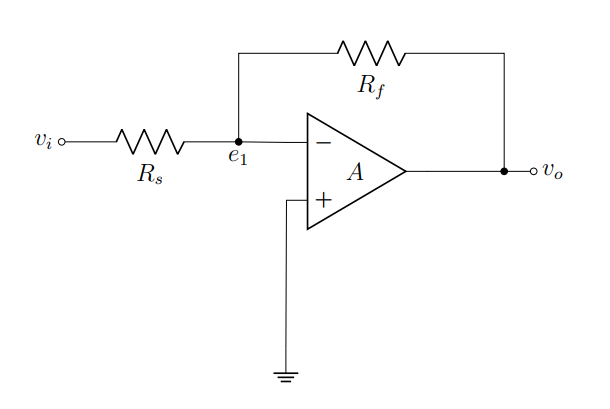
\includegraphics[width=0.5\textwidth]{src/images/amplificador-inversor.png}
    \caption{Amplificador inversor}
    \label{fig:mt-amplificador-inversor}
\end{figure}

\begin{figure}[ht]
    \centering
    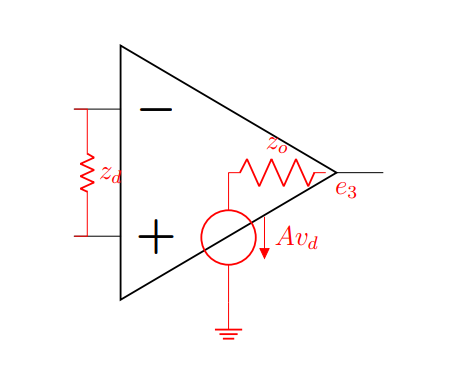
\includegraphics[width=0.5\textwidth]{src/images/modelo-amp-base.png}
    \caption{Modelo de amplificador base}
    \label{fig:mt-modelo-amp-base}
\end{figure}


Aplicando el Método de Amplificador Desvanecido al amplificador inversor, tomando en cuenta los modelos de las figuras 2.2 y 2.3, se tiene

\begin{align*}
    x_{i0} &= \left. \frac{v_o}{v_i} \right|_{A=0} = \frac{(R_f + z_o) \parallel z_d}{R_s + (R_f + z_o) \parallel z_d} \cdot \frac{z_o}{z_o + R_f} \\
    x_{i1} &= \left. \frac{e_1}{v_i} \right|_{A=0} = \frac{(R_f + z_o) \parallel z_d}{R_s + (R_f + z_o) \parallel z_d} \\
    x_{3o} &= \left. \frac{v_o}{e_3} \right|_{v_i=0} = \frac{R_f + R_s \parallel z_d}{z_o + R_f + R_s \parallel z_d} \\
    x_{31} &= \left. \frac{e_1}{e_3} \right|_{v_i=0} = \frac{R_s \parallel z_d}{z_o + R_f + R_s \parallel z_d}
\end{align*}

Ahora, aproximando la impedancia de entrada y salida $Z_d \rightarrow \infty $ y $z_o \rightarrow 0$ entonces:

\begin{align*}
x_{i0} &= \left. \frac{v_o}{v_i} \right|_{A=0} = 0 \\
x_{i1} &= \left. \frac{e_1}{v_i} \right|_{A=0} = -\frac{R_f}{R_s + R_f} \\
x_{3o} &= \left. \frac{v_o}{e_3} \right|_{v_i=0} = 1 \\
x_{31} &= \left. \frac{e_1}{e_3} \right|_{v_i=0} = -\frac{R_s}{R_f + R_s}
\end{align*}

Aplicando la fórmula MAD se tiene: 

\begin{equation*}
A_{fb} = 0 + \frac{-\frac{R_f}{R_s + R_f} \cdot A \cdot 1}{1 - \left( -\frac{R_s}{R_f + R_s} \right) A} \\
\end{equation*}

\begin{equation}
    \boxed{A_{fb} = -\frac{R_f}{R_s}}
    \label{eq:mt-ganancia-amp-inversor}
\end{equation}


Por otro lado, la impedancia de entrada se busca utilizando el teorema de Blackman.

\begin{align*}
z_a &= R_s \parallel z_d + R_f = R_s + R_f \\
x_{31cc} &= -\frac{R_s \parallel z_d}{R_f + R_s \parallel z_d} = -\frac{R_s}{R_f + R_s} \\
x_{31ca} &= -\frac{z_d}{z_d + R_f} \approx -1
\end{align*}


Por lo tanto, aplicando la formula 

\begin{equation*}
z_{in} = (R_s + R_f) \cdot \frac{1 - \left( \frac{-R_s}{R_f + R_s} \right) A}{1 - (-1)A} \\
\end{equation*}

Tomando $A \rightarrow \infty$ 

\begin{equation}
    \boxed{z_{in} = R_s}
\end{equation}

Por último, también utilizamos la fórmula de blackman para encontrar la impedancia de salida.

\begin{align*}
z_a &= r_o \parallel (R_f + R_s \parallel z_d) = r_o \\
x_{31cc} &= 0 \\
x_{31ca} &= -\frac{R_s \parallel z_d}{R_f + R_s \parallel z_d} = -\frac{R_s}{R_f + R_s} \\
z_o &= r_o \cdot \frac{1 - 0}{1 - \left( -\frac{R_s}{R_f + R_s} \right) A} 
\end{align*}

Lo cual se puede escribir como:

\begin{equation}
\boxed{z_o = \frac{r_o}{A / \left( 1 + \frac{R_f}{R_s} \right)}}
\end{equation}

\subsection{Amplificador no inversor}

Al igual que el amplificador inversor, este es uno de las topologías básicas de los amplificadores operacionales. Este amplificador se muestra en la figura \ref{fig:mt-amp-no-inversor}, cuya diferencia radica en que la entrada ahora es directamente en el puerto no inversor.

\begin{figure}[ht]
    \centering
    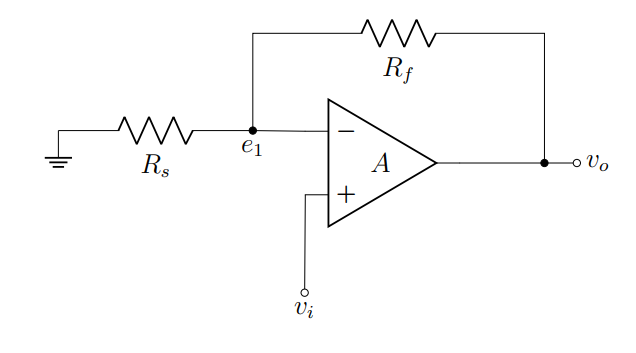
\includegraphics[width=0.5\textwidth]{src/images/amp-no-inversor.png}
    \caption{Amplificador no inversor}
    \label{fig:mt-amp-no-inversor}
\end{figure}

Aplicando el Método de Amplificador Desvanecido y aproximando la impedancia de entrada y salida $z_d \rightarrow \infty$ y $z_o \rightarrow 0$, entonces

\begin{align*}
x_{i0} &= \left. \frac{v_o}{v_i} \right|_{A=0} = 0 \\
x_{i1} &= \left. \frac{e_1}{v_i} \right|_{A=0} = 1 \\
x_{3o} &= \left. \frac{v_o}{e_3} \right|_{v_i=0} = 1 \\
x_{31} &= \left. \frac{e_1}{e_3} \right|_{v_i=0} = -\frac{R_s}{R_f + R_s}
\end{align*}


Por lo tanto, aplicando la fórmula de MAD

\begin{align*}
A_{fb} &= 0 + \frac{1 \cdot A \cdot 1}{1 - \left( -\frac{R_s}{R_f + R_s} \right) A} \\
\end{align*}

\begin{equation}
    \boxed{A_{fb} = 1 + \frac{R_f}{R_s}}
    \label{eq:mt-ganancia-amp-no-inversor}
\end{equation}

Por otro lado, la impedancia de entrada se busca utilizando el Teorema de Blackman.

\begin{align*}
z_a &= z_d + R_s \parallel R_f = z_d \\
x_{31cc} &= \frac{-R_s \parallel z_d}{R_f + R_s \parallel z_d} = \frac{-R_s}{R_f + R_s} \\
x_{31ca} &= 0
\end{align*}

Donde este último es nulo debido que al abrir el circuito no pasa corriente por $z_d$, por consiguiente no habrá tensión.

\begin{align*}
z_{in} &= z_d \cdot \frac{1 - \left( \frac{-R_s}{R_f + R_s} \right) A}{1 - 0 \cdot A} \\
\end{align*}

\begin{equation}
    \boxed{z_{in} = z_d \cdot \frac{ A}{1 + \frac{R_f}{R_s}}}
\end{equation}


Por último, calculamos la impedancia de salida, la cual será igual a la
impedancia de salida del amplificador inversor.

\begin{equation}
\boxed{z_o = \frac{r_o}{A / \left( 1 + \frac{R_f}{R_s} \right)}}
\end{equation}


\subsection{Amplificador en diferencia o restador}

La siguiente aplicación corresponde al amplificador en diferencia, el cual
tiene una salida y dos entradas, una aplicada a la entrada inversora y otra a la
entrada no inversora. La salida es una combinación lineal de las entradas. Por
otro lado las resistencias vistas desde sus entradas son finitas y diferentes la
una de la otra. Si las fuentes de entrada son diferentes, entonces se producirá
un efecto de carga distinto debido a la diferencia entre estas impedancias.

\begin{figure}[ht]
    \centering
    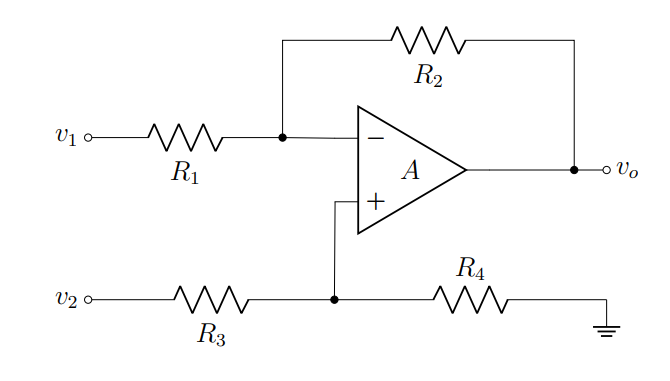
\includegraphics[width=0.5\textwidth]{src/images/amp-restador.png}
    \caption{Amplificador en diferencia o restador}
    \label{fig:mt-amp-restador}
\end{figure}

El amplificador en diferencia es un circuito que responde sólo al componente en modo diferencial, rechazando el componente en modo común.

\begin{align*}
v_o &= -\frac{R_2}{R_1} v_1 + \frac{R_4}{R_3 + R_4} \cdot \left( 1 + \frac{R_2}{R_1} \right) v_2 \\
v_o &= -\frac{R_2}{R_1} v_1 + \frac{R_4}{R_3 + R_4} \cdot \left( \frac{R_1 + R_2}{R_1} \right) v_2
\end{align*}

Para este caso particular, si $R_1 = R_4$ y $R_2 = R_3$, entonces se puede
simplificar

\begin{equation}
    \boxed{v_o = \frac{R_2}{R_1} (v_2 - v_1)}
    \label{eq:mt-ganancia-restador}
\end{equation}

Sin embargo, existe una diferencia entre las impedancias de entrada.

\begin{align*}
z_{in1} &= R_1 \\
z_{in2} &= R_3 + R_4 = R_1 + R_2
\end{align*}


Un amplificador en diferencia será insensible a la tensión en modo común,
a medida que el amplificador sea ideal y que las resistencias cumplan la
condición de puente balanceado.

\subsection{Amplificador integrador}

Si se sustituye la resistencia de realimentación Rf por un condensador en un amplificador inversor, entonces tendremos un integrador. Se puede demostrar que la función de transferencia es

\begin{align*}
\frac{v_o}{v_i} &= -\frac{1}{sRC}
\end{align*}

Si se apaga la tensión $v_i$ en el integrador, este estará influenciado solo por la acción de la tensión y la crriente de offset. Estudiando sólo la tensión de offset, se tiene que el voltaje de salida es:

\begin{align*}
v_o &= v_{os} + \frac{t}{RC} v_{os}
\end{align*}

Por lo tanto, se puede observar que la tensión de salida crecerá hasta que se sature el amplificador. Un comportamiento similar ocurre por la acción de la corrientes de bias.

\begin{align*}
v_o &= -I_{b2}R + \left( I_{b1} - \frac{I_{b2}R}{R} \right) \frac{t}{C}
\end{align*}

\subsection{Convertidor de tensión a corriente}

El circuito consiste en una fuente de entrada $V_i$ con una resistencia en serie $R_1$, y un convertidor de resistencia negativa que sintetiza una resistencia a tierra de valor $-R_2 R_3 / R_4$ como en la figura \ref{fig:mt-fuente-corriente-howland}.

\begin{figure}
    \centering
    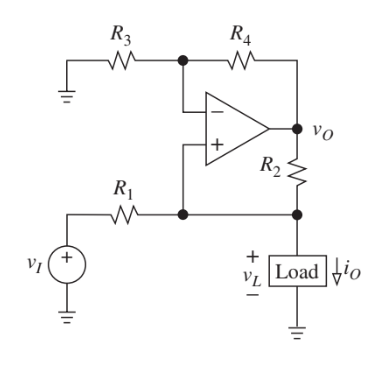
\includegraphics[width=0.5\textwidth]{src/images/fuente-corriente-howland.png}
    \caption{Fuente de corriente de Howland}
    \label{fig:mt-fuente-corriente-howland}
\end{figure}

Podemos simplificar el circuito aplicando Blackman tomando parte del cirtuito cómo un amplificador no inversor:

\begin{align*}
    z & = z_a \cdot \frac{1 - X_{3icc}A}{1 - X_{3ica}A} \\
    z_a & = R_1 \parallel R_2 \\
    X_{31cc} Q& = \left. \frac{e_1}{e_3} \right|_{v_a=0} \\
\end{align*}

al utilizar la formula de MAD, obtenemos la ganancia:

\begin{equation}
    A_1 = 1 + \frac{R_2}{R_1}
\end{equation}

Podemos aproximar la impedancia de entrada y salida $Z_d \rightarrow \infty $ y $z_o \rightarrow 0$ y obtener el nuevo circuito simplificado de la figura \ref{fig:mt-fuente-corriente-howland-simplificado}.

\begin{figure}[ht]
    \centering
    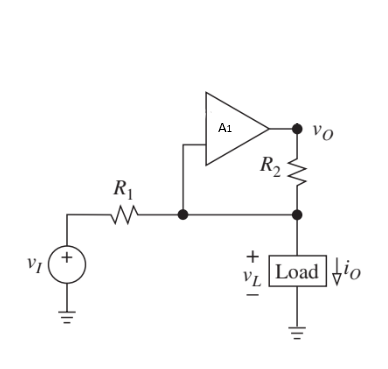
\includegraphics[width=0.5\textwidth]{src/images/fuente-corriente-howland-simplificado.png}
    \caption{Fuente de corriente de Howland simplificada}
    \label{fig:mt-fuente-corriente-howland-simplificado}    
\end{figure}

Aplicando nuevamente Blackman en el circuito simplificado:

\begin{align*}
    X_{31ca} = \left. \frac{e_1}{e_3} \right|_{I_a=0} = \frac{R_1}{R_1 + R_2} \\
    z_o = R_1 \parallel R_2 (\frac{1 - 0A}{1 - \frac{R_1}{R_1 + R_2}(1 + \frac{R_4}{R_3})}) \\
    z_o = \frac{R_1 R_2 / R_1 + R_2}{\frac{R_3(R_1 + R_2) - R_1(R_3 + R_4)}{(R_1 + R_2)R_3}} \\
\end{align*}

resultando en:

\begin{equation}
    z_o = \frac{R_1 R_2 R_3}{R_2 R_3 - R_1 R_4}
\end{equation}

para que $Z_o \rightarrow\infty$ el denominador debe ser igual a 0:

\begin{align*}
    R_2 R_3 - R_1 R_4 = 0 \\
    R_2 R_3 = R_1 R_4
\end{align*}

por lo que 

\begin{align}
    \boxed{R_1 = R_3} \\
    \boxed{R_2 = R_4} 
\end{align}

Cuando se cumple esta condición, la salida se vuelve independiente de $V_l$:

\begin{equation}
    \boxed{i_o = \frac{1}{R1} V_i}
    \label{eq:mt-io-fuente-corriente}
\end{equation}

Dado que $V_L = V_o \frac{R_3}{R_3 + R_4} = V_o \frac{R_1}{R_1 + R_2}$, el máximo  voltaje de salida para actuar en la zona lineal es, asumiendo una saturación de salida simétrica,  

\begin{equation}
    \left| V_L \right| \leq  \frac{R_1}{R_1 + R_2} V_{sat}
\end{equation}

Para el proposito de extender el rango de linealidad, es deseable mantener $R_2$ suficientemente pequeño en comparación	con $R_1$ (por ejemplo, $R_2 \approx 0.1 R_1$).